\documentclass[runningheads,a4paper]{article}

\usepackage[utf8]{inputenc}
 
\setcounter{tocdepth}{3}

\usepackage[english]{babel} 
\usepackage{graphicx}
\usepackage{grffile}
\usepackage{float}
\usepackage{multicol}
\usepackage{url}
\usepackage{array}
\usepackage{wrapfig}
\usepackage{multirow}
\usepackage{tabu}
\usepackage{amssymb}% http://ctan.org/pkg/amssymb
\usepackage{pifont}% http://ctan.org/pkg/pifont
\usepackage[font=small,labelfont=bf]{caption}

\newcommand{\cmark}{\ding{51}}%
\newcommand{\xmark}{\ding{55}}%
 
\usepackage{titling}
\usepackage[hidelinks]{hyperref}
\setcounter{secnumdepth}{5}
%Margins
\usepackage[
margin=2cm,
includefoot
]{geometry}


\graphicspath{{/}}

%Headers and Footers
\usepackage{fancyhdr}
\pagestyle{fancy}
\fancyhead{}
\fancyfoot{}
\fancyfoot[R]{\thepage}
\renewcommand{\headrulewidth}{0pt}
\renewcommand{\footrulewidth}{0pt}
 \setlength\parindent{24pt}
\begin{document}

	%Title Page
	\begin{titlepage}
		\begin{center}
			
\includegraphics[width=10cm]{fig/UP.jpg}  \\
			[1cm]
			\line(1,0){300} \\
			[0.3cm]
			\textsc{\Large
				NavUP\\
				Testing Report\\
			\hfill
				%University of Pretoria
			}\\
			[0.1cm]
			\line(1,0){300} \\
			[0.7cm]
			\textsc{\Large
				Andriod-GIS
			} \\
		\end{center}
		
		\begin{center}
			\begin{multicols}{2}
				\textsc{\large\\
				Mfana Masimula\\ 
					12077713\\ 
				}
				
				\textsc{\large\\
				Joshua Moodley\\
					 14152152\\ 
				}
				
			\textsc{\large\\
				Bongani Tshela\\ 
				14134790\\ 
			}
			
			\textsc{\large\\
				Boikanyo Modiko\\
				15227678\\ 
			}
		
			\end{multicols}
			
			
			\textsc{\\ \href{https://github.com/SirJosh/Android-GIS}{GitHub}
				\url{https://github.com/SirJosh/Android-GIS.git}}
		\end{center}
	\end{titlepage}
%\maketitle

\begingroup

\tableofcontents
\addcontentsline{toc}{section}{Table Of Contents}
\endgroup
\newpage

\section{Introduction}

\subsection{Scope}
Services to gather, maintain, persist and provide information related to the world
serviced by the system. It is about the creation and maintenance of a GIS Map of the
campus by using WiFi signal strengths and other available sources of GIS
information.
This module provide services to search for locations such as landmarks, buildings as
well as venues such as offices, lecture halls, labs, etc.
 
\section{Functional Requirements}
\subsection{Create Functionality}
\subsubsection{Add a location}

\label{my-label}
\begin{tabular}{|l|l|l|l|}
	\hline
	\textbf{Pass/Fail} & \textbf{Mark (10)} & \multicolumn{2}{l|}{\textbf{Reason}}                                                                                                                                                              \\ 
	\hline
	\cmark  &   8  & \multicolumn{2}{l|}{\begin{tabular}[c]{@{}l@{}}this is some text that is a lot of text can you -lease wraparound \\ so it omdfshjvafkdghjvnadhjkvbknadf\\vjh,kandfb vadfbadfbsf\end{tabular}} \\ \hline
\end{tabular}

\subsection{Remove Functionality}
\subsubsection{Remove location}

\begin{tabular}{|l|l|l|l|}
	\hline
	\textbf{Pass/Fail} & \textbf{Mark (10)} & \multicolumn{2}{l|}{\textbf{Reason}}                                                                                                                                                              \\ 
	\hline
	\cmark  &   8  & \multicolumn{2}{l|}{\begin{tabular}[c]{@{}l@{}}this is some text that is a lot of text can you -lease wraparound \\ so it omdfshjvafkdghjvnadhjkvbknadf\\vjh,kandfb vadfbadfbsf\end{tabular}} \\ \hline
\end{tabular}

\subsection{Update Functionality}
\subsubsection{Update location}

\begin{tabular}{|l|l|l|l|}
	\hline
	\textbf{Pass/Fail} & \textbf{Mark (10)} & \multicolumn{2}{l|}{\textbf{Reason}}                                                                                                                                                              \\ 
	\hline
	\cmark  &   8  & \multicolumn{2}{l|}{\begin{tabular}[c]{@{}l@{}}this is some text that is a lot of text can you -lease wraparound \\ so it omdfshjvafkdghjvnadhjkvbknadf\\vjh,kandfb vadfbadfbsf\end{tabular}} \\ \hline
\end{tabular}

\pagebreak
\subsection{Request Functionality}
\subsubsection{Get all locations}
\begin{tabular}{|l|l|l|l|}
	\hline
	\textbf{Pass/Fail} & \textbf{Mark (10)} & \multicolumn{2}{l|}{\textbf{Reason}}                                                                                                                                                              \\ 
	\hline
		\cmark &  8  & \multicolumn{2}{l|}{\begin{tabular}[c]{@{}l@{}}The retrieve all locations request returns all the location's stored within the \\ database on campus. The request works when new locations are added. Thus \\ showing that the database performs the request correctly. This also holds true \\ when you call this function multiple times sequentially. \\ \\ Overall the function performs what it is defined to do, without causing  strain on \\the database.\end{tabular}} \\ \hline
\end{tabular}

\begin{center}
\begin{minipage}{0.48\linewidth}
	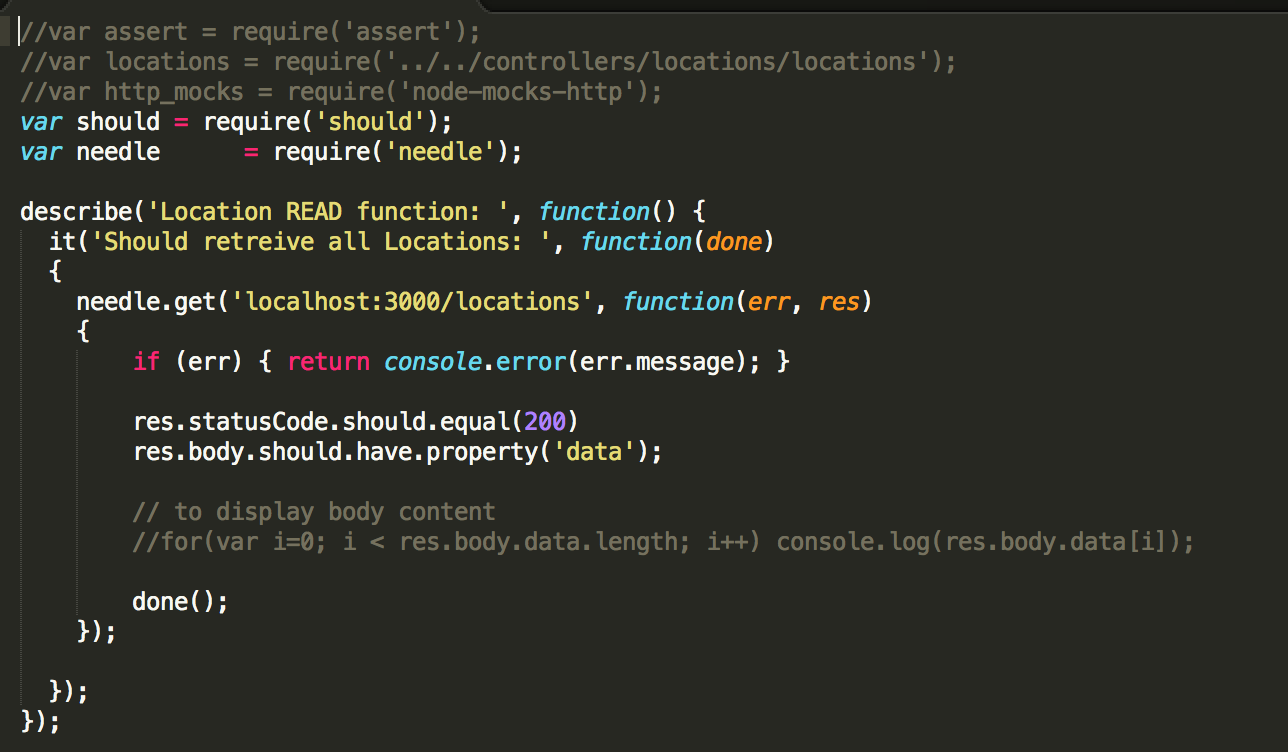
\includegraphics[width=\linewidth]{fig/allLocationCode.png}
	\captionof{figure}{Test code for display all locations}
\end{minipage}
\hfill
\begin{minipage}{0.49\linewidth}
	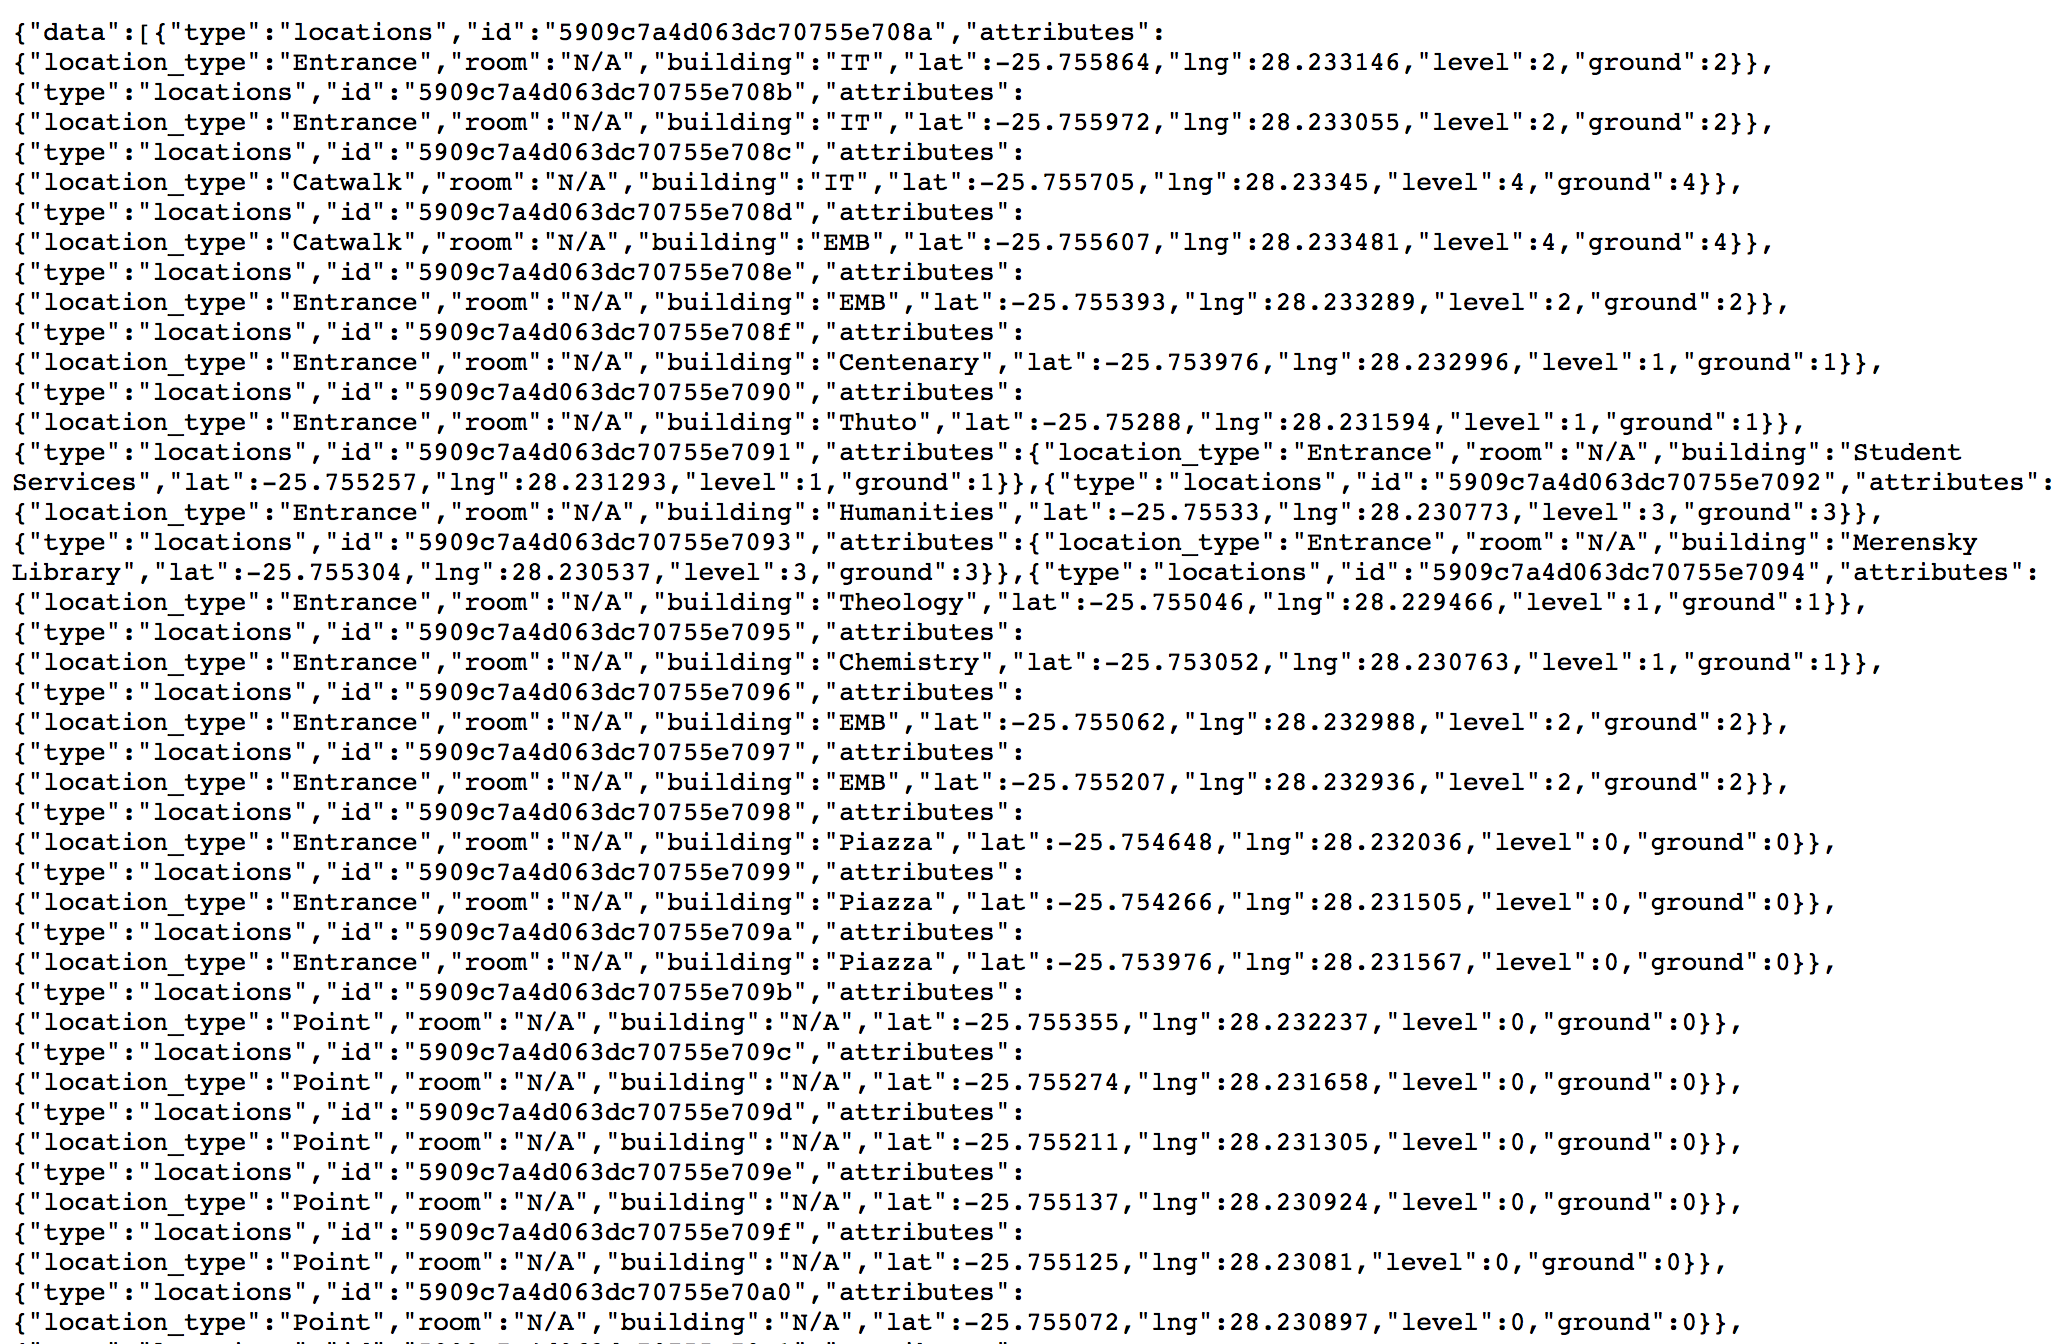
\includegraphics[width=\linewidth]{fig/allLocationResult.png}
	\captionof{figure}{JSON string returned}
\end{minipage}
\begin{minipage}{0.40\linewidth}
	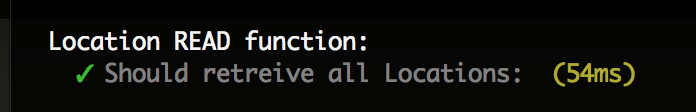
\includegraphics[width=\linewidth]{fig/allLocationTerm.png}
	\captionof{figure}{Result after test is run: status code 200}
\end{minipage}
\end{center}


\subsubsection{Get all buildings}
\begin{tabular}{|l|l|l|l|}
	\hline
	\textbf{Pass/Fail} & \textbf{Mark (10)} & \multicolumn{2}{l|}{\textbf{Reason}}                                                                                                                                                              \\ 
	\hline
		\cmark &  8  & \multicolumn{2}{l|}{\begin{tabular}[c]{@{}l@{}}After testing the getBuildingNames request it retrieves all the buildings that are \\ on campus. The request also works when new buildings are added. Thus showing \\ that the database handles the request correctly. This also holds true when you call \\ this function multiple times sequentially. \\ \\ Overall the function performs what it needs to do, without causing the database to  \\ crash or hang.\end{tabular}} \\ \hline
	
\end{tabular}

\begin{center}
	\begin{minipage}{0.48\linewidth}
		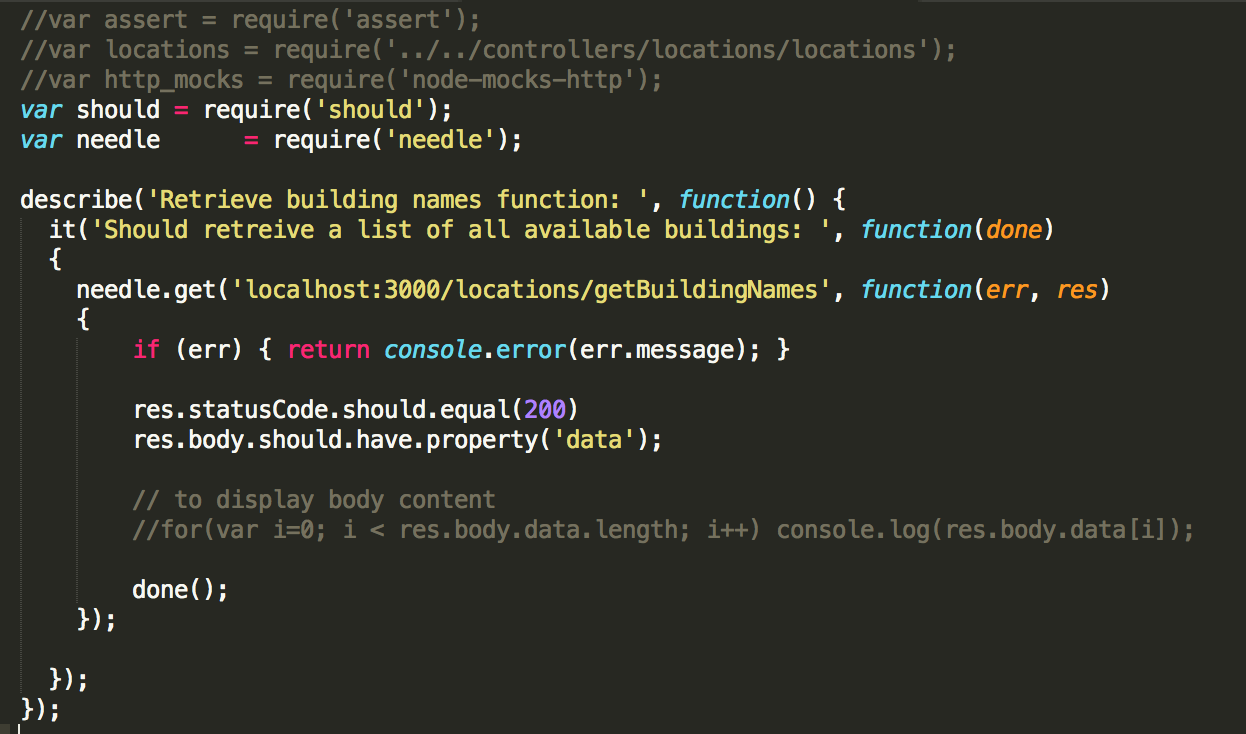
\includegraphics[width=\linewidth]{fig/buildingSearch.png}
		\captionof{figure}{Test code for display all function}
	\end{minipage}
	\hfill
	\begin{minipage}{0.49\linewidth}
		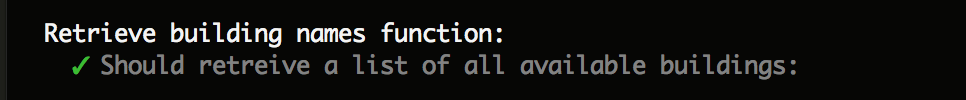
\includegraphics[width=\linewidth]{fig/ReqBuildAll.png}
		\captionof{figure}{Result after test is run: status code 200}
	\end{minipage}
	\begin{minipage}{1.0\linewidth}
		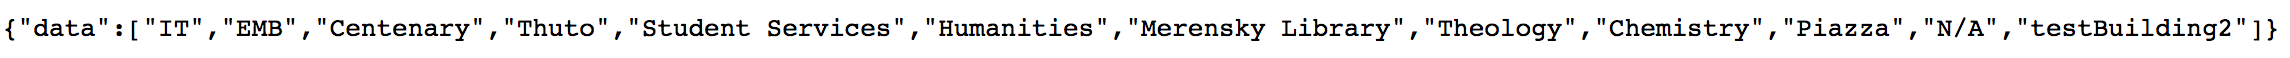
\includegraphics[width=\linewidth]{fig/buildalldata.png}
		\captionof{figure}{JSON string returned}
	\end{minipage}
\end{center}




\subsubsection{Get location by building name}
\begin{tabular}{|l|l|l|l|}
	\hline
	\textbf{Pass/Fail} & \textbf{Mark (10)} & \multicolumn{2}{l|}{\textbf{Reason}}                                                                                                                                                              \\ 
	\hline
	\cmark  &   8  & \multicolumn{2}{l|}{\begin{tabular}[c]{@{}l@{}}this is some text that is a lot of text can you -lease wraparound \\ so it omdfshjvafkdghjvnadhjkvbknadf\\vjh,kandfb vadfbadfbsf\end{tabular}} \\ \hline
\end{tabular}

\subsubsection{Get route}
\begin{tabular}{|l|l|l|l|}
	\hline
	\textbf{Pass/Fail} & \textbf{Mark (10)} & \multicolumn{2}{l|}{\textbf{Reason}}                                                                                                                                                              \\ 
	\hline
	\cmark  &   8  & \multicolumn{2}{l|}{\begin{tabular}[c]{@{}l@{}}this is some text that is a lot of text can you -lease wraparound \\ so it omdfshjvafkdghjvnadhjkvbknadf\\vjh,kandfb vadfbadfbsf\end{tabular}} \\ \hline
\end{tabular}

\section{Non-Functional Requirements Tested}
\subsection{Reliability}
\begin{tabular}{|l|l|l|l|}
	\hline
	\textbf{Pass/Fail} & \textbf{Mark (10)} & \multicolumn{2}{l|}{\textbf{Reason}}                                                                                                                                                              \\ 
	\hline
	\cmark  &   8  & \multicolumn{2}{l|}{\begin{tabular}[c]{@{}l@{}}this is some text that is a lot of text can you -lease wraparound \\ so it omdfshjvafkdghjvnadhjkvbknadf\\vjh,kandfb vadfbadfbsf\end{tabular}} \\ \hline
\end{tabular}

\subsection{Availability}
\begin{tabular}{|l|l|l|l|}
	\hline
	\textbf{Pass/Fail} & \textbf{Mark (10)} & \multicolumn{2}{l|}{\textbf{Reason}}                                                                                                                                                              \\ 
	\hline
	\cmark  &   8  & \multicolumn{2}{l|}{\begin{tabular}[c]{@{}l@{}}this is some text that is a lot of text can you -lease wraparound \\ so it omdfshjvafkdghjvnadhjkvbknadf\\vjh,kandfb vadfbadfbsf\end{tabular}} \\ \hline
\end{tabular}

\subsection{Scalability}
\begin{tabular}{|l|l|l|l|}
	\hline
	\textbf{Pass/Fail} & \textbf{Mark (10)} & \multicolumn{2}{l|}{\textbf{Reason}}                                                                                                                                                              \\ 
	\hline
	\cmark  &   8  & \multicolumn{2}{l|}{\begin{tabular}[c]{@{}l@{}}this is some text that is a lot of text can you -lease wraparound \\ so it omdfshjvafkdghjvnadhjkvbknadf\\vjh,kandfb vadfbadfbsf\end{tabular}} \\ \hline
\end{tabular}

\subsection{Recoverability}
\begin{tabular}{|l|l|l|l|}
	\hline
	\textbf{Pass/Fail} & \textbf{Mark (10)} & \multicolumn{2}{l|}{\textbf{Reason}}                                                                                                                                                              \\ 
	\hline
	\cmark  &   8  & \multicolumn{2}{l|}{\begin{tabular}[c]{@{}l@{}}this is some text that is a lot of text can you -lease wraparound \\ so it omdfshjvafkdghjvnadhjkvbknadf\\vjh,kandfb vadfbadfbsf\end{tabular}} \\ \hline
\end{tabular}

\end{document}